% slides for neo-presention
\documentclass{beamer}

\usepackage[ngerman]{babel}
\usepackage[utf8]{inputenc}
\usepackage[]{color}


\usetheme{Copenhagen}

\setbeamercovered{transparent}
\beamertemplatenavigationsymbolsempty
\setbeamertemplate{footline}[frame number]
\setbeamertemplate{sections/subsections in toc}[default]

\usecolortheme{seahorse}

\titlegraphic{
\includegraphics[width=4cm]{images/logo.png}}

\title{NEO - Ergonomisch optimiert}

\author[M. Schmidinger]{
    Markus Schmidinger
}

\begin{document}

\begin{frame}[plain]
  \titlepage
\end{frame}

\frame[plain]{
  \frametitle{Inhaltsverzeichnis}
  \tableofcontents
  [hideallsubsections]
}

\section{Geschichte}

\subsection{QWERTY}
\frame[<+->]{
  \begin{itemize}
    \item QWERTY/QWERTZ
    \item entwickelt 1868, zum Schreiben auf mechanischen Tastaturen
    \item keinerlei ergonomische Optimierung
  \end{itemize}
}

\subsection{ergonomische Layouts}
\frame[<+->]{
  \begin{itemize}
    \item 1932: Dvorak 
    \item optimiert für die englische Sprache
    \item gibt auch eine deutsche Variante
  \end{itemize}
  \begin{figure}[p]
    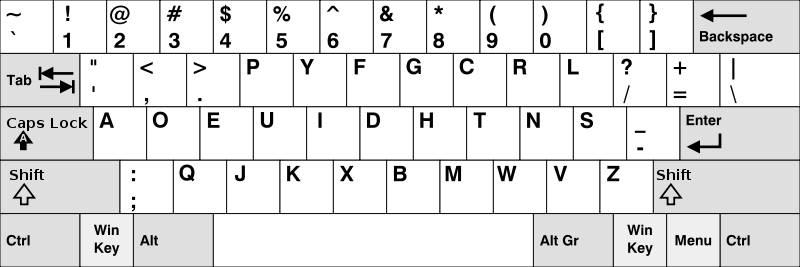
\includegraphics[width=8cm]{images/dvorak.png}
  \end{figure}
}
\frame[<+->]{
  \begin{itemize}
    \item 2003: de-ergo
    \item 2004: neo1
    \item 2010: neo2
  \end{itemize}
}

\section{Umsetzung}
\frame[<+->]{
  \begin{itemize}
    \item Häufige Verwendung der Grundlinie
    \item Buchstabenpaare, die am häufigsten aufeinander folgen auf 2 Hände verteilt
    \item stärkere Belastung auf Zeige- und Mittelfinger
    \item Gleiche Verteilung auf linke und rechte Hand
    \item Optimierung für Deutsch, Englisch, Programmiersprachen, Shell-Befehle
    \item Sonderzeichen für Programmierung sind gut erreichbar
    \item mathematische Symbole können einfach eingegeben werden
    \item Ziffernblock, Steuerkreuz auf eigener Ebene
  \end{itemize}
}

\section{Ebenen}
\subsection{1}\frame[label=Ebene1]{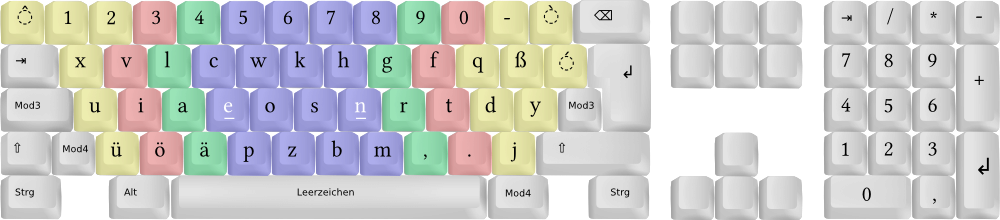
\includegraphics[width=\linewidth]{images/neo_ebene1.png}}
\subsection{2}\frame[label=Ebene2]{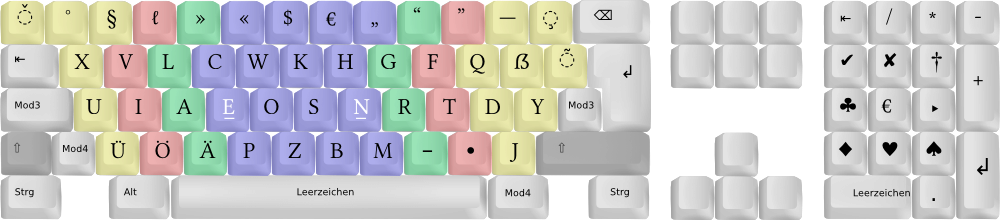
\includegraphics[width=\linewidth]{images/neo_ebene2.png}}
\subsection{3}\frame[label=Ebene3]{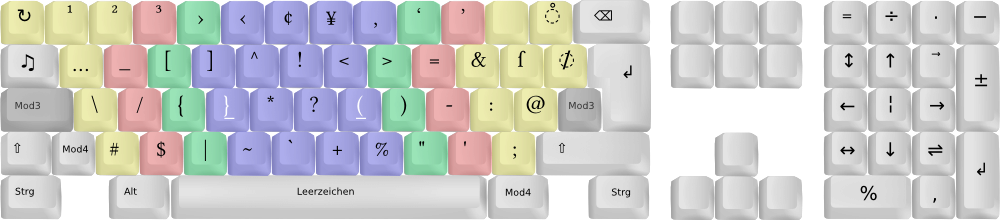
\includegraphics[width=\linewidth]{images/neo_ebene3.png}}

\subsection{4}\frame[label=Ebene4]{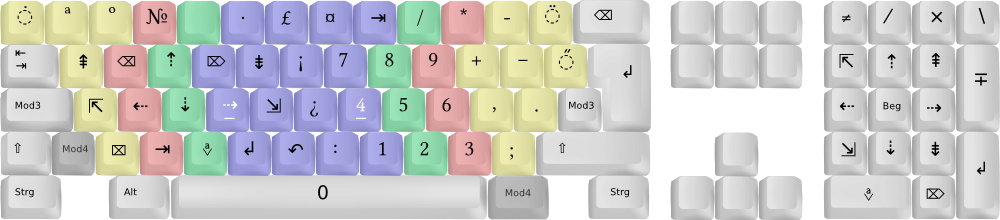
\includegraphics[width=\linewidth]{images/neo_ebene4.png}}
\subsection{5}\frame[label=Ebene5]{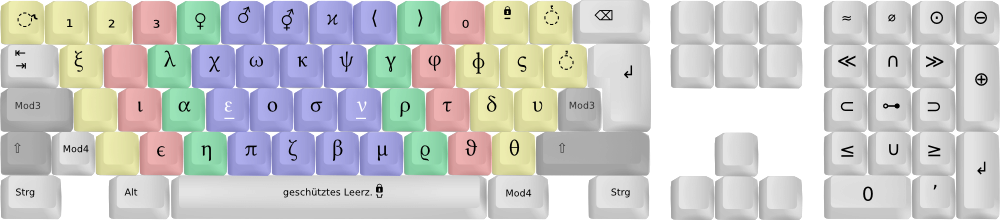
\includegraphics[width=\linewidth]{images/neo_ebene5.png}}
\subsection{6}\frame[label=Ebene6]{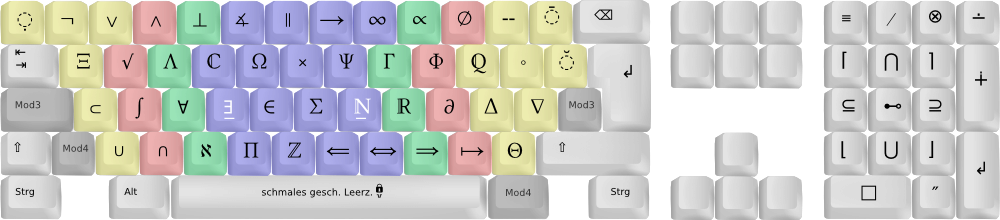
\includegraphics[width=\linewidth]{images/neo_ebene6.png}}

\section{Vergleich Homerow}
\subsection{NEO}
\frame{
  \textcolor{green}{A}\textcolor{red}{l}\textcolor{green}{s} \textcolor{red}{L}\textcolor{green}{i}\textcolor{green}{n}\textcolor{green}{u}\textcolor{red}{x} \textcolor{green}{o}\textcolor{green}{d}\textcolor{green}{e}\textcolor{green}{r} \textcolor{red}{G}\textcolor{green}{N}\textcolor{green}{U}\textcolor{red}{/}\textcolor{red}{L}\textcolor{green}{i}\textcolor{green}{n}\textcolor{green}{u}\textcolor{red}{x} \textcolor{red}{(}\textcolor{green}{s}\textcolor{green}{i}\textcolor{green}{e}\textcolor{red}{h}\textcolor{green}{e} \textcolor{red}{G}\textcolor{green}{N}\textcolor{green}{U}\textcolor{red}{/}\textcolor{red}{L}\textcolor{green}{i}\textcolor{green}{n}\textcolor{green}{u}\textcolor{red}{x}\textcolor{red}{-}\textcolor{green}{N}\textcolor{green}{a}\textcolor{red}{m}\textcolor{green}{e}\textcolor{green}{n}\textcolor{green}{s}\textcolor{green}{s}\textcolor{green}{t}\textcolor{green}{r}\textcolor{green}{e}\textcolor{green}{i}\textcolor{green}{t}\textcolor{red}{)} \textcolor{red}{b}\textcolor{green}{e}\textcolor{red}{z}\textcolor{green}{e}\textcolor{green}{i}\textcolor{red}{c}\textcolor{red}{h}\textcolor{green}{n}\textcolor{green}{e}\textcolor{green}{t} \textcolor{red}{m}\textcolor{green}{a}\textcolor{green}{n} \textcolor{green}{i}\textcolor{green}{n} \textcolor{green}{d}\textcolor{green}{e}\textcolor{green}{r} \textcolor{green}{R}\textcolor{green}{e}\textcolor{red}{g}\textcolor{green}{e}\textcolor{red}{l} \textcolor{red}{f}\textcolor{green}{r}\textcolor{green}{e}\textcolor{green}{i}\textcolor{green}{e}\textcolor{red}{,} \textcolor{green}{u}\textcolor{green}{n}\textcolor{green}{i}\textcolor{red}{x}\textcolor{red}{-}\textcolor{red}{ä}\textcolor{red}{h}\textcolor{green}{n}\textcolor{red}{l}\textcolor{green}{i}\textcolor{red}{c}\textcolor{red}{h}\textcolor{green}{e} \textcolor{red}{M}\textcolor{green}{e}\textcolor{red}{h}\textcolor{green}{r}\textcolor{red}{b}\textcolor{green}{e}\textcolor{green}{n}\textcolor{green}{u}\textcolor{green}{t}\textcolor{red}{z}\textcolor{green}{e}\textcolor{green}{r}\textcolor{red}{-}\textcolor{red}{B}\textcolor{green}{e}\textcolor{green}{t}\textcolor{green}{r}\textcolor{green}{i}\textcolor{green}{e}\textcolor{red}{b}\textcolor{green}{s}\textcolor{green}{s}\textcolor{green}{y}\textcolor{green}{s}\textcolor{green}{t}\textcolor{green}{e}\textcolor{red}{m}\textcolor{green}{e}\textcolor{red}{,} \textcolor{green}{d}\textcolor{green}{i}\textcolor{green}{e} \textcolor{green}{a}\textcolor{green}{u}\textcolor{red}{f} \textcolor{green}{d}\textcolor{green}{e}\textcolor{red}{m} \textcolor{red}{L}\textcolor{green}{i}\textcolor{green}{n}\textcolor{green}{u}\textcolor{red}{x}\textcolor{red}{-}\textcolor{red}{K}\textcolor{green}{e}\textcolor{green}{r}\textcolor{green}{n}\textcolor{green}{e}\textcolor{red}{l} \textcolor{green}{u}\textcolor{green}{n}\textcolor{green}{d} \textcolor{red}{w}\textcolor{green}{e}\textcolor{green}{s}\textcolor{green}{e}\textcolor{green}{n}\textcolor{green}{t}\textcolor{red}{l}\textcolor{green}{i}\textcolor{red}{c}\textcolor{red}{h} \textcolor{green}{a}\textcolor{green}{u}\textcolor{red}{f} \textcolor{red}{G}\textcolor{green}{N}\textcolor{green}{U}\textcolor{red}{-}\textcolor{green}{S}\textcolor{green}{o}\textcolor{red}{f}\textcolor{green}{t}\textcolor{red}{w}\textcolor{green}{a}\textcolor{green}{r}\textcolor{green}{e} \textcolor{red}{b}\textcolor{green}{a}\textcolor{green}{s}\textcolor{green}{i}\textcolor{green}{e}\textcolor{green}{r}\textcolor{green}{e}\textcolor{green}{n}\textcolor{red}{.} \textcolor{green}{D}\textcolor{green}{i}\textcolor{green}{e} \textcolor{red}{w}\textcolor{green}{e}\textcolor{green}{i}\textcolor{green}{t}\textcolor{green}{e}\textcolor{red}{,} \textcolor{green}{a}\textcolor{green}{u}\textcolor{red}{c}\textcolor{red}{h} \textcolor{red}{k}\textcolor{green}{o}\textcolor{red}{m}\textcolor{red}{m}\textcolor{green}{e}\textcolor{green}{r}\textcolor{red}{z}\textcolor{green}{i}\textcolor{green}{e}\textcolor{red}{l}\textcolor{red}{l}\textcolor{green}{e} \textcolor{red}{V}\textcolor{green}{e}\textcolor{green}{r}\textcolor{red}{b}\textcolor{green}{r}\textcolor{green}{e}\textcolor{green}{i}\textcolor{green}{t}\textcolor{green}{u}\textcolor{green}{n}\textcolor{red}{g} \textcolor{red}{w}\textcolor{green}{u}\textcolor{green}{r}\textcolor{green}{d}\textcolor{green}{e} \textcolor{green}{a}\textcolor{red}{b} \textcolor{red}{1}\textcolor{red}{9}\textcolor{red}{9}\textcolor{red}{2} \textcolor{green}{d}\textcolor{green}{u}\textcolor{green}{r}\textcolor{red}{c}\textcolor{red}{h} \textcolor{green}{d}\textcolor{green}{i}\textcolor{green}{e} \textcolor{red}{L}\textcolor{green}{i}\textcolor{red}{z}\textcolor{green}{e}\textcolor{green}{n}\textcolor{red}{z}\textcolor{green}{i}\textcolor{green}{e}\textcolor{green}{r}\textcolor{green}{u}\textcolor{green}{n}\textcolor{red}{g} \textcolor{green}{d}\textcolor{green}{e}\textcolor{green}{s} \textcolor{red}{L}\textcolor{green}{i}\textcolor{green}{n}\textcolor{green}{u}\textcolor{red}{x}\textcolor{red}{-}\textcolor{red}{K}\textcolor{green}{e}\textcolor{green}{r}\textcolor{green}{n}\textcolor{green}{e}\textcolor{red}{l}\textcolor{green}{s} \textcolor{green}{u}\textcolor{green}{n}\textcolor{green}{t}\textcolor{green}{e}\textcolor{green}{r} \textcolor{green}{d}\textcolor{green}{e}\textcolor{green}{r} \textcolor{red}{f}\textcolor{green}{r}\textcolor{green}{e}\textcolor{green}{i}\textcolor{green}{e}\textcolor{green}{n} \textcolor{red}{L}\textcolor{green}{i}\textcolor{red}{z}\textcolor{green}{e}\textcolor{green}{n}\textcolor{red}{z} \textcolor{red}{G}\textcolor{red}{P}\textcolor{red}{L} \textcolor{green}{e}\textcolor{green}{r}\textcolor{red}{m}\textcolor{red}{ö}\textcolor{red}{g}\textcolor{red}{l}\textcolor{green}{i}\textcolor{red}{c}\textcolor{red}{h}\textcolor{green}{t}\textcolor{red}{.}\textcolor{red}{
}\textcolor{green}{D}\textcolor{green}{a}\textcolor{green}{s} \textcolor{red}{m}\textcolor{green}{o}\textcolor{green}{d}\textcolor{green}{u}\textcolor{red}{l}\textcolor{green}{a}\textcolor{green}{r} \textcolor{green}{a}\textcolor{green}{u}\textcolor{red}{f}\textcolor{red}{g}\textcolor{green}{e}\textcolor{red}{b}\textcolor{green}{a}\textcolor{green}{u}\textcolor{green}{t}\textcolor{green}{e} \textcolor{red}{B}\textcolor{green}{e}\textcolor{green}{t}\textcolor{green}{r}\textcolor{green}{i}\textcolor{green}{e}\textcolor{red}{b}\textcolor{green}{s}\textcolor{green}{s}\textcolor{green}{y}\textcolor{green}{s}\textcolor{green}{t}\textcolor{green}{e}\textcolor{red}{m} \textcolor{red}{w}\textcolor{green}{i}\textcolor{green}{r}\textcolor{green}{d} \textcolor{red}{v}\textcolor{green}{o}\textcolor{green}{n} \textcolor{green}{S}\textcolor{green}{o}\textcolor{red}{f}\textcolor{green}{t}\textcolor{red}{w}\textcolor{green}{a}\textcolor{green}{r}\textcolor{green}{e}\textcolor{green}{e}\textcolor{green}{n}\textcolor{green}{t}\textcolor{red}{w}\textcolor{green}{i}\textcolor{red}{c}\textcolor{red}{k}\textcolor{red}{l}\textcolor{green}{e}\textcolor{green}{r}\textcolor{green}{n} \textcolor{green}{a}\textcolor{green}{u}\textcolor{red}{f} \textcolor{green}{d}\textcolor{green}{e}\textcolor{green}{r} \textcolor{red}{g}\textcolor{green}{a}\textcolor{green}{n}\textcolor{red}{z}\textcolor{green}{e}\textcolor{green}{n} \textcolor{red}{W}\textcolor{green}{e}\textcolor{red}{l}\textcolor{green}{t} \textcolor{red}{w}\textcolor{green}{e}\textcolor{green}{i}\textcolor{green}{t}\textcolor{green}{e}\textcolor{green}{r}\textcolor{green}{e}\textcolor{green}{n}\textcolor{green}{t}\textcolor{red}{w}\textcolor{green}{i}\textcolor{red}{c}\textcolor{red}{k}\textcolor{green}{e}\textcolor{red}{l}\textcolor{green}{t}\textcolor{red}{,} \textcolor{green}{d}\textcolor{green}{i}\textcolor{green}{e} \textcolor{green}{a}\textcolor{green}{n} \textcolor{green}{d}\textcolor{green}{e}\textcolor{green}{n} \textcolor{red}{v}\textcolor{green}{e}\textcolor{green}{r}\textcolor{green}{s}\textcolor{red}{c}\textcolor{red}{h}\textcolor{green}{i}\textcolor{green}{e}\textcolor{green}{d}\textcolor{green}{e}\textcolor{green}{n}\textcolor{green}{e}\textcolor{green}{n} \textcolor{red}{P}\textcolor{green}{r}\textcolor{green}{o}\textcolor{red}{j}\textcolor{green}{e}\textcolor{red}{k}\textcolor{green}{t}\textcolor{green}{e}\textcolor{green}{n} \textcolor{red}{m}\textcolor{green}{i}\textcolor{green}{t}\textcolor{green}{a}\textcolor{green}{r}\textcolor{red}{b}\textcolor{green}{e}\textcolor{green}{i}\textcolor{green}{t}\textcolor{green}{e}\textcolor{green}{n}\textcolor{red}{.} \textcolor{green}{A}\textcolor{green}{n} \textcolor{green}{d}\textcolor{green}{e}\textcolor{green}{r} \textcolor{green}{E}\textcolor{green}{n}\textcolor{green}{t}\textcolor{red}{w}\textcolor{green}{i}\textcolor{red}{c}\textcolor{red}{k}\textcolor{red}{l}\textcolor{green}{u}\textcolor{green}{n}\textcolor{red}{g} \textcolor{green}{s}\textcolor{green}{i}\textcolor{green}{n}\textcolor{green}{d} \textcolor{green}{U}\textcolor{green}{n}\textcolor{green}{t}\textcolor{green}{e}\textcolor{green}{r}\textcolor{green}{n}\textcolor{green}{e}\textcolor{red}{h}\textcolor{red}{m}\textcolor{green}{e}\textcolor{green}{n}\textcolor{red}{,} \textcolor{green}{N}\textcolor{green}{o}\textcolor{green}{n}\textcolor{red}{-}\textcolor{red}{P}\textcolor{green}{r}\textcolor{green}{o}\textcolor{red}{f}\textcolor{green}{i}\textcolor{green}{t}\textcolor{red}{-}\textcolor{green}{O}\textcolor{green}{r}\textcolor{red}{g}\textcolor{green}{a}\textcolor{green}{n}\textcolor{green}{i}\textcolor{green}{s}\textcolor{green}{a}\textcolor{green}{t}\textcolor{green}{i}\textcolor{green}{o}\textcolor{green}{n}\textcolor{green}{e}\textcolor{green}{n} \textcolor{green}{u}\textcolor{green}{n}\textcolor{green}{d} \textcolor{red}{v}\textcolor{green}{i}\textcolor{green}{e}\textcolor{red}{l}\textcolor{green}{e} \textcolor{red}{F}\textcolor{green}{r}\textcolor{green}{e}\textcolor{green}{i}\textcolor{red}{w}\textcolor{green}{i}\textcolor{red}{l}\textcolor{red}{l}\textcolor{green}{i}\textcolor{red}{g}\textcolor{green}{e} \textcolor{red}{b}\textcolor{green}{e}\textcolor{green}{t}\textcolor{green}{e}\textcolor{green}{i}\textcolor{red}{l}\textcolor{green}{i}\textcolor{red}{g}\textcolor{green}{t}\textcolor{red}{.} \textcolor{red}{B}\textcolor{green}{e}\textcolor{green}{i}\textcolor{red}{m} \textcolor{red}{G}\textcolor{green}{e}\textcolor{red}{b}\textcolor{green}{r}\textcolor{green}{a}\textcolor{green}{u}\textcolor{red}{c}\textcolor{red}{h} \textcolor{green}{a}\textcolor{green}{u}\textcolor{red}{f} \textcolor{red}{C}\textcolor{green}{o}\textcolor{red}{m}\textcolor{red}{p}\textcolor{green}{u}\textcolor{green}{t}\textcolor{green}{e}\textcolor{green}{r}\textcolor{green}{n} \textcolor{red}{k}\textcolor{green}{o}\textcolor{red}{m}\textcolor{red}{m}\textcolor{green}{e}\textcolor{green}{n} \textcolor{red}{m}\textcolor{green}{e}\textcolor{green}{i}\textcolor{green}{s}\textcolor{green}{t} \textcolor{green}{s}\textcolor{green}{o}\textcolor{red}{g}\textcolor{green}{e}\textcolor{green}{n}\textcolor{green}{a}\textcolor{green}{n}\textcolor{green}{n}\textcolor{green}{t}\textcolor{green}{e} \textcolor{red}{L}\textcolor{green}{i}\textcolor{green}{n}\textcolor{green}{u}\textcolor{red}{x}\textcolor{red}{-}\textcolor{green}{D}\textcolor{green}{i}\textcolor{green}{s}\textcolor{green}{t}\textcolor{green}{r}\textcolor{green}{i}\textcolor{red}{b}\textcolor{green}{u}\textcolor{green}{t}\textcolor{green}{i}\textcolor{green}{o}\textcolor{green}{n}\textcolor{green}{e}\textcolor{green}{n} \textcolor{red}{z}\textcolor{green}{u}\textcolor{red}{m} \textcolor{green}{E}\textcolor{green}{i}\textcolor{green}{n}\textcolor{green}{s}\textcolor{green}{a}\textcolor{green}{t}\textcolor{red}{z}\textcolor{red}{.} \textcolor{green}{E}\textcolor{green}{i}\textcolor{green}{n}\textcolor{green}{e} \textcolor{green}{D}\textcolor{green}{i}\textcolor{green}{s}\textcolor{green}{t}\textcolor{green}{r}\textcolor{green}{i}\textcolor{red}{b}\textcolor{green}{u}\textcolor{green}{t}\textcolor{green}{i}\textcolor{green}{o}\textcolor{green}{n} \textcolor{red}{f}\textcolor{green}{a}\textcolor{green}{s}\textcolor{green}{s}\textcolor{green}{t} \textcolor{green}{d}\textcolor{green}{e}\textcolor{green}{n} \textcolor{red}{L}\textcolor{green}{i}\textcolor{green}{n}\textcolor{green}{u}\textcolor{red}{x}\textcolor{red}{-}\textcolor{red}{K}\textcolor{green}{e}\textcolor{green}{r}\textcolor{green}{n}\textcolor{green}{e}\textcolor{red}{l} \textcolor{red}{m}\textcolor{green}{i}\textcolor{green}{t} \textcolor{red}{v}\textcolor{green}{e}\textcolor{green}{r}\textcolor{green}{s}\textcolor{red}{c}\textcolor{red}{h}\textcolor{green}{i}\textcolor{green}{e}\textcolor{green}{d}\textcolor{green}{e}\textcolor{green}{n}\textcolor{green}{e}\textcolor{green}{r} \textcolor{green}{S}\textcolor{green}{o}\textcolor{red}{f}\textcolor{green}{t}\textcolor{red}{w}\textcolor{green}{a}\textcolor{green}{r}\textcolor{green}{e} \textcolor{red}{z}\textcolor{green}{u} \textcolor{green}{e}\textcolor{green}{i}\textcolor{green}{n}\textcolor{green}{e}\textcolor{red}{m} \textcolor{red}{B}\textcolor{green}{e}\textcolor{green}{t}\textcolor{green}{r}\textcolor{green}{i}\textcolor{green}{e}\textcolor{red}{b}\textcolor{green}{s}\textcolor{green}{s}\textcolor{green}{y}\textcolor{green}{s}\textcolor{green}{t}\textcolor{green}{e}\textcolor{red}{m} \textcolor{red}{z}\textcolor{green}{u}\textcolor{green}{s}\textcolor{green}{a}\textcolor{red}{m}\textcolor{red}{m}\textcolor{green}{e}\textcolor{green}{n}\textcolor{red}{,} \textcolor{green}{d}\textcolor{green}{a}\textcolor{green}{s} \textcolor{red}{f}\textcolor{red}{ü}\textcolor{green}{r} \textcolor{green}{d}\textcolor{green}{i}\textcolor{green}{e} \textcolor{green}{E}\textcolor{green}{n}\textcolor{green}{d}\textcolor{green}{n}\textcolor{green}{u}\textcolor{green}{t}\textcolor{red}{z}\textcolor{green}{u}\textcolor{green}{n}\textcolor{red}{g} \textcolor{red}{g}\textcolor{green}{e}\textcolor{green}{e}\textcolor{green}{i}\textcolor{red}{g}\textcolor{green}{n}\textcolor{green}{e}\textcolor{green}{t} \textcolor{green}{i}\textcolor{green}{s}\textcolor{green}{t}\textcolor{red}{.}\textcolor{red}{
}
}

\subsection{QWERTZ}
\frame{ 
  \textcolor{green}{A}\textcolor{green}{l}\textcolor{green}{s} \textcolor{green}{L}\textcolor{red}{i}\textcolor{red}{n}\textcolor{red}{u}\textcolor{red}{x} \textcolor{red}{o}\textcolor{green}{d}\textcolor{red}{e}\textcolor{red}{r} \textcolor{green}{G}\textcolor{red}{N}\textcolor{red}{U}\textcolor{red}{/}\textcolor{green}{L}\textcolor{red}{i}\textcolor{red}{n}\textcolor{red}{u}\textcolor{red}{x} \textcolor{red}{(}\textcolor{green}{s}\textcolor{red}{i}\textcolor{red}{e}\textcolor{green}{h}\textcolor{red}{e} \textcolor{green}{G}\textcolor{red}{N}\textcolor{red}{U}\textcolor{red}{/}\textcolor{green}{L}\textcolor{red}{i}\textcolor{red}{n}\textcolor{red}{u}\textcolor{red}{x}\textcolor{red}{-}\textcolor{red}{N}\textcolor{green}{a}\textcolor{red}{m}\textcolor{red}{e}\textcolor{red}{n}\textcolor{green}{s}\textcolor{green}{s}\textcolor{red}{t}\textcolor{red}{r}\textcolor{red}{e}\textcolor{red}{i}\textcolor{red}{t}\textcolor{red}{)} \textcolor{red}{b}\textcolor{red}{e}\textcolor{red}{z}\textcolor{red}{e}\textcolor{red}{i}\textcolor{red}{c}\textcolor{green}{h}\textcolor{red}{n}\textcolor{red}{e}\textcolor{red}{t} \textcolor{red}{m}\textcolor{green}{a}\textcolor{red}{n} \textcolor{red}{i}\textcolor{red}{n} \textcolor{green}{d}\textcolor{red}{e}\textcolor{red}{r} \textcolor{red}{R}\textcolor{red}{e}\textcolor{green}{g}\textcolor{red}{e}\textcolor{green}{l} \textcolor{green}{f}\textcolor{red}{r}\textcolor{red}{e}\textcolor{red}{i}\textcolor{red}{e}\textcolor{red}{,} \textcolor{red}{u}\textcolor{red}{n}\textcolor{red}{i}\textcolor{red}{x}\textcolor{red}{-}\textcolor{green}{ä}\textcolor{green}{h}\textcolor{red}{n}\textcolor{green}{l}\textcolor{red}{i}\textcolor{red}{c}\textcolor{green}{h}\textcolor{red}{e} \textcolor{red}{M}\textcolor{red}{e}\textcolor{green}{h}\textcolor{red}{r}\textcolor{red}{b}\textcolor{red}{e}\textcolor{red}{n}\textcolor{red}{u}\textcolor{red}{t}\textcolor{red}{z}\textcolor{red}{e}\textcolor{red}{r}\textcolor{red}{-}\textcolor{red}{B}\textcolor{red}{e}\textcolor{red}{t}\textcolor{red}{r}\textcolor{red}{i}\textcolor{red}{e}\textcolor{red}{b}\textcolor{green}{s}\textcolor{green}{s}\textcolor{red}{y}\textcolor{green}{s}\textcolor{red}{t}\textcolor{red}{e}\textcolor{red}{m}\textcolor{red}{e}\textcolor{red}{,} \textcolor{green}{d}\textcolor{red}{i}\textcolor{red}{e} \textcolor{green}{a}\textcolor{red}{u}\textcolor{green}{f} \textcolor{green}{d}\textcolor{red}{e}\textcolor{red}{m} \textcolor{green}{L}\textcolor{red}{i}\textcolor{red}{n}\textcolor{red}{u}\textcolor{red}{x}\textcolor{red}{-}\textcolor{green}{K}\textcolor{red}{e}\textcolor{red}{r}\textcolor{red}{n}\textcolor{red}{e}\textcolor{green}{l} \textcolor{red}{u}\textcolor{red}{n}\textcolor{green}{d} \textcolor{red}{w}\textcolor{red}{e}\textcolor{green}{s}\textcolor{red}{e}\textcolor{red}{n}\textcolor{red}{t}\textcolor{green}{l}\textcolor{red}{i}\textcolor{red}{c}\textcolor{green}{h} \textcolor{green}{a}\textcolor{red}{u}\textcolor{green}{f} \textcolor{green}{G}\textcolor{red}{N}\textcolor{red}{U}\textcolor{red}{-}\textcolor{green}{S}\textcolor{red}{o}\textcolor{green}{f}\textcolor{red}{t}\textcolor{red}{w}\textcolor{green}{a}\textcolor{red}{r}\textcolor{red}{e} \textcolor{red}{b}\textcolor{green}{a}\textcolor{green}{s}\textcolor{red}{i}\textcolor{red}{e}\textcolor{red}{r}\textcolor{red}{e}\textcolor{red}{n}\textcolor{red}{.} \textcolor{green}{D}\textcolor{red}{i}\textcolor{red}{e} \textcolor{red}{w}\textcolor{red}{e}\textcolor{red}{i}\textcolor{red}{t}\textcolor{red}{e}\textcolor{red}{,} \textcolor{green}{a}\textcolor{red}{u}\textcolor{red}{c}\textcolor{green}{h} \textcolor{green}{k}\textcolor{red}{o}\textcolor{red}{m}\textcolor{red}{m}\textcolor{red}{e}\textcolor{red}{r}\textcolor{red}{z}\textcolor{red}{i}\textcolor{red}{e}\textcolor{green}{l}\textcolor{green}{l}\textcolor{red}{e} \textcolor{red}{V}\textcolor{red}{e}\textcolor{red}{r}\textcolor{red}{b}\textcolor{red}{r}\textcolor{red}{e}\textcolor{red}{i}\textcolor{red}{t}\textcolor{red}{u}\textcolor{red}{n}\textcolor{green}{g} \textcolor{red}{w}\textcolor{red}{u}\textcolor{red}{r}\textcolor{green}{d}\textcolor{red}{e} \textcolor{green}{a}\textcolor{red}{b} \textcolor{red}{1}\textcolor{red}{9}\textcolor{red}{9}\textcolor{red}{2} \textcolor{green}{d}\textcolor{red}{u}\textcolor{red}{r}\textcolor{red}{c}\textcolor{green}{h} \textcolor{green}{d}\textcolor{red}{i}\textcolor{red}{e} \textcolor{green}{L}\textcolor{red}{i}\textcolor{red}{z}\textcolor{red}{e}\textcolor{red}{n}\textcolor{red}{z}\textcolor{red}{i}\textcolor{red}{e}\textcolor{red}{r}\textcolor{red}{u}\textcolor{red}{n}\textcolor{green}{g} \textcolor{green}{d}\textcolor{red}{e}\textcolor{green}{s} \textcolor{green}{L}\textcolor{red}{i}\textcolor{red}{n}\textcolor{red}{u}\textcolor{red}{x}\textcolor{red}{-}\textcolor{green}{K}\textcolor{red}{e}\textcolor{red}{r}\textcolor{red}{n}\textcolor{red}{e}\textcolor{green}{l}\textcolor{green}{s} \textcolor{red}{u}\textcolor{red}{n}\textcolor{red}{t}\textcolor{red}{e}\textcolor{red}{r} \textcolor{green}{d}\textcolor{red}{e}\textcolor{red}{r} \textcolor{green}{f}\textcolor{red}{r}\textcolor{red}{e}\textcolor{red}{i}\textcolor{red}{e}\textcolor{red}{n} \textcolor{green}{L}\textcolor{red}{i}\textcolor{red}{z}\textcolor{red}{e}\textcolor{red}{n}\textcolor{red}{z} \textcolor{green}{G}\textcolor{red}{P}\textcolor{green}{L} \textcolor{red}{e}\textcolor{red}{r}\textcolor{red}{m}\textcolor{green}{ö}\textcolor{green}{g}\textcolor{green}{l}\textcolor{red}{i}\textcolor{red}{c}\textcolor{green}{h}\textcolor{red}{t}\textcolor{red}{.}\textcolor{red}{
}\textcolor{green}{D}\textcolor{green}{a}\textcolor{green}{s} \textcolor{red}{m}\textcolor{red}{o}\textcolor{green}{d}\textcolor{red}{u}\textcolor{green}{l}\textcolor{green}{a}\textcolor{red}{r} \textcolor{green}{a}\textcolor{red}{u}\textcolor{green}{f}\textcolor{green}{g}\textcolor{red}{e}\textcolor{red}{b}\textcolor{green}{a}\textcolor{red}{u}\textcolor{red}{t}\textcolor{red}{e} \textcolor{red}{B}\textcolor{red}{e}\textcolor{red}{t}\textcolor{red}{r}\textcolor{red}{i}\textcolor{red}{e}\textcolor{red}{b}\textcolor{green}{s}\textcolor{green}{s}\textcolor{red}{y}\textcolor{green}{s}\textcolor{red}{t}\textcolor{red}{e}\textcolor{red}{m} \textcolor{red}{w}\textcolor{red}{i}\textcolor{red}{r}\textcolor{green}{d} \textcolor{red}{v}\textcolor{red}{o}\textcolor{red}{n} \textcolor{green}{S}\textcolor{red}{o}\textcolor{green}{f}\textcolor{red}{t}\textcolor{red}{w}\textcolor{green}{a}\textcolor{red}{r}\textcolor{red}{e}\textcolor{red}{e}\textcolor{red}{n}\textcolor{red}{t}\textcolor{red}{w}\textcolor{red}{i}\textcolor{red}{c}\textcolor{green}{k}\textcolor{green}{l}\textcolor{red}{e}\textcolor{red}{r}\textcolor{red}{n} \textcolor{green}{a}\textcolor{red}{u}\textcolor{green}{f} \textcolor{green}{d}\textcolor{red}{e}\textcolor{red}{r} \textcolor{green}{g}\textcolor{green}{a}\textcolor{red}{n}\textcolor{red}{z}\textcolor{red}{e}\textcolor{red}{n} \textcolor{red}{W}\textcolor{red}{e}\textcolor{green}{l}\textcolor{red}{t} \textcolor{red}{w}\textcolor{red}{e}\textcolor{red}{i}\textcolor{red}{t}\textcolor{red}{e}\textcolor{red}{r}\textcolor{red}{e}\textcolor{red}{n}\textcolor{red}{t}\textcolor{red}{w}\textcolor{red}{i}\textcolor{red}{c}\textcolor{green}{k}\textcolor{red}{e}\textcolor{green}{l}\textcolor{red}{t}\textcolor{red}{,} \textcolor{green}{d}\textcolor{red}{i}\textcolor{red}{e} \textcolor{green}{a}\textcolor{red}{n} \textcolor{green}{d}\textcolor{red}{e}\textcolor{red}{n} \textcolor{red}{v}\textcolor{red}{e}\textcolor{red}{r}\textcolor{green}{s}\textcolor{red}{c}\textcolor{green}{h}\textcolor{red}{i}\textcolor{red}{e}\textcolor{green}{d}\textcolor{red}{e}\textcolor{red}{n}\textcolor{red}{e}\textcolor{red}{n} \textcolor{red}{P}\textcolor{red}{r}\textcolor{red}{o}\textcolor{green}{j}\textcolor{red}{e}\textcolor{green}{k}\textcolor{red}{t}\textcolor{red}{e}\textcolor{red}{n} \textcolor{red}{m}\textcolor{red}{i}\textcolor{red}{t}\textcolor{green}{a}\textcolor{red}{r}\textcolor{red}{b}\textcolor{red}{e}\textcolor{red}{i}\textcolor{red}{t}\textcolor{red}{e}\textcolor{red}{n}\textcolor{red}{.} \textcolor{green}{A}\textcolor{red}{n} \textcolor{green}{d}\textcolor{red}{e}\textcolor{red}{r} \textcolor{red}{E}\textcolor{red}{n}\textcolor{red}{t}\textcolor{red}{w}\textcolor{red}{i}\textcolor{red}{c}\textcolor{green}{k}\textcolor{green}{l}\textcolor{red}{u}\textcolor{red}{n}\textcolor{green}{g} \textcolor{green}{s}\textcolor{red}{i}\textcolor{red}{n}\textcolor{green}{d} \textcolor{red}{U}\textcolor{red}{n}\textcolor{red}{t}\textcolor{red}{e}\textcolor{red}{r}\textcolor{red}{n}\textcolor{red}{e}\textcolor{green}{h}\textcolor{red}{m}\textcolor{red}{e}\textcolor{red}{n}\textcolor{red}{,} \textcolor{red}{N}\textcolor{red}{o}\textcolor{red}{n}\textcolor{red}{-}\textcolor{red}{P}\textcolor{red}{r}\textcolor{red}{o}\textcolor{green}{f}\textcolor{red}{i}\textcolor{red}{t}\textcolor{red}{-}\textcolor{red}{O}\textcolor{red}{r}\textcolor{green}{g}\textcolor{green}{a}\textcolor{red}{n}\textcolor{red}{i}\textcolor{green}{s}\textcolor{green}{a}\textcolor{red}{t}\textcolor{red}{i}\textcolor{red}{o}\textcolor{red}{n}\textcolor{red}{e}\textcolor{red}{n} \textcolor{red}{u}\textcolor{red}{n}\textcolor{green}{d} \textcolor{red}{v}\textcolor{red}{i}\textcolor{red}{e}\textcolor{green}{l}\textcolor{red}{e} \textcolor{green}{F}\textcolor{red}{r}\textcolor{red}{e}\textcolor{red}{i}\textcolor{red}{w}\textcolor{red}{i}\textcolor{green}{l}\textcolor{green}{l}\textcolor{red}{i}\textcolor{green}{g}\textcolor{red}{e} \textcolor{red}{b}\textcolor{red}{e}\textcolor{red}{t}\textcolor{red}{e}\textcolor{red}{i}\textcolor{green}{l}\textcolor{red}{i}\textcolor{green}{g}\textcolor{red}{t}\textcolor{red}{.} \textcolor{red}{B}\textcolor{red}{e}\textcolor{red}{i}\textcolor{red}{m} \textcolor{green}{G}\textcolor{red}{e}\textcolor{red}{b}\textcolor{red}{r}\textcolor{green}{a}\textcolor{red}{u}\textcolor{red}{c}\textcolor{green}{h} \textcolor{green}{a}\textcolor{red}{u}\textcolor{green}{f} \textcolor{red}{C}\textcolor{red}{o}\textcolor{red}{m}\textcolor{red}{p}\textcolor{red}{u}\textcolor{red}{t}\textcolor{red}{e}\textcolor{red}{r}\textcolor{red}{n} \textcolor{green}{k}\textcolor{red}{o}\textcolor{red}{m}\textcolor{red}{m}\textcolor{red}{e}\textcolor{red}{n} \textcolor{red}{m}\textcolor{red}{e}\textcolor{red}{i}\textcolor{green}{s}\textcolor{red}{t} \textcolor{green}{s}\textcolor{red}{o}\textcolor{green}{g}\textcolor{red}{e}\textcolor{red}{n}\textcolor{green}{a}\textcolor{red}{n}\textcolor{red}{n}\textcolor{red}{t}\textcolor{red}{e} \textcolor{green}{L}\textcolor{red}{i}\textcolor{red}{n}\textcolor{red}{u}\textcolor{red}{x}\textcolor{red}{-}\textcolor{green}{D}\textcolor{red}{i}\textcolor{green}{s}\textcolor{red}{t}\textcolor{red}{r}\textcolor{red}{i}\textcolor{red}{b}\textcolor{red}{u}\textcolor{red}{t}\textcolor{red}{i}\textcolor{red}{o}\textcolor{red}{n}\textcolor{red}{e}\textcolor{red}{n} \textcolor{red}{z}\textcolor{red}{u}\textcolor{red}{m} \textcolor{red}{E}\textcolor{red}{i}\textcolor{red}{n}\textcolor{green}{s}\textcolor{green}{a}\textcolor{red}{t}\textcolor{red}{z}\textcolor{red}{.} \textcolor{red}{E}\textcolor{red}{i}\textcolor{red}{n}\textcolor{red}{e} \textcolor{green}{D}\textcolor{red}{i}\textcolor{green}{s}\textcolor{red}{t}\textcolor{red}{r}\textcolor{red}{i}\textcolor{red}{b}\textcolor{red}{u}\textcolor{red}{t}\textcolor{red}{i}\textcolor{red}{o}\textcolor{red}{n} \textcolor{green}{f}\textcolor{green}{a}\textcolor{green}{s}\textcolor{green}{s}\textcolor{red}{t} \textcolor{green}{d}\textcolor{red}{e}\textcolor{red}{n} \textcolor{green}{L}\textcolor{red}{i}\textcolor{red}{n}\textcolor{red}{u}\textcolor{red}{x}\textcolor{red}{-}\textcolor{green}{K}\textcolor{red}{e}\textcolor{red}{r}\textcolor{red}{n}\textcolor{red}{e}\textcolor{green}{l} \textcolor{red}{m}\textcolor{red}{i}\textcolor{red}{t} \textcolor{red}{v}\textcolor{red}{e}\textcolor{red}{r}\textcolor{green}{s}\textcolor{red}{c}\textcolor{green}{h}\textcolor{red}{i}\textcolor{red}{e}\textcolor{green}{d}\textcolor{red}{e}\textcolor{red}{n}\textcolor{red}{e}\textcolor{red}{r} \textcolor{green}{S}\textcolor{red}{o}\textcolor{green}{f}\textcolor{red}{t}\textcolor{red}{w}\textcolor{green}{a}\textcolor{red}{r}\textcolor{red}{e} \textcolor{red}{z}\textcolor{red}{u} \textcolor{red}{e}\textcolor{red}{i}\textcolor{red}{n}\textcolor{red}{e}\textcolor{red}{m} \textcolor{red}{B}\textcolor{red}{e}\textcolor{red}{t}\textcolor{red}{r}\textcolor{red}{i}\textcolor{red}{e}\textcolor{red}{b}\textcolor{green}{s}\textcolor{green}{s}\textcolor{red}{y}\textcolor{green}{s}\textcolor{red}{t}\textcolor{red}{e}\textcolor{red}{m} \textcolor{red}{z}\textcolor{red}{u}\textcolor{green}{s}\textcolor{green}{a}\textcolor{red}{m}\textcolor{red}{m}\textcolor{red}{e}\textcolor{red}{n}\textcolor{red}{,} \textcolor{green}{d}\textcolor{green}{a}\textcolor{green}{s} \textcolor{green}{f}\textcolor{red}{ü}\textcolor{red}{r} \textcolor{green}{d}\textcolor{red}{i}\textcolor{red}{e} \textcolor{red}{E}\textcolor{red}{n}\textcolor{green}{d}\textcolor{red}{n}\textcolor{red}{u}\textcolor{red}{t}\textcolor{red}{z}\textcolor{red}{u}\textcolor{red}{n}\textcolor{green}{g} \textcolor{green}{g}\textcolor{red}{e}\textcolor{red}{e}\textcolor{red}{i}\textcolor{green}{g}\textcolor{red}{n}\textcolor{red}{e}\textcolor{red}{t} \textcolor{red}{i}\textcolor{green}{s}\textcolor{red}{t}\textcolor{red}{.}\textcolor{red}{
}
}

\end{document}
